\documentclass[a4paper,10pt]{article}
\usepackage[left=1in,right=1in,top=1in,bottom=1in]{geometry}
\usepackage[english,russian]{babel}
\usepackage{enumitem}
\usepackage[hidelinks]{hyperref}
\usepackage{titlesec}
\usepackage{multirow}
\usepackage{graphicx}
\usepackage{wrapfig}
\usepackage{tabularx}
\usepackage{float}
\usepackage{longtable}
\usepackage{hyperref}
\hypersetup{colorlinks=true,urlcolor=blue}
\usepackage[rgb]{xcolor}
\usepackage{amsmath,amsfonts,amssymb,amsthm,mathtools} 
\usepackage{icomma} 
\mathtoolsset{showonlyrefs=true}
\usepackage{euscript}
\usepackage{mathrsfs}
\usepackage{setspace}
\usepackage{cmap}          
\usepackage{mathtext}         
\usepackage[T2A]{fontenc}      
\usepackage[utf8]{inputenc}      

\titleformat{\section}{\Large\bfseries}{}{0em}{}[\titlerule]
\pagestyle{empty}

\begin{document}

\begin{center}
    \textbf{\LARGE Даниэль Александрович Сахаров} \\
    \vspace{5pt}
    \href{https://github.com/grgtr}{GitHub} $\vert$
    sakharov.da@phystech.edu $\vert$ 
    tg: @xxxgrgtr
\end{center}

\section*{Образование}
\noindent
\textbf{МФТИ} \hfill 2022 - 2026
Высшая школа программной инженерии ИВТ

\section*{Опыт работы}
\noindent
\subsection*{Стажёр отдела Big Data MTS, банковый скоринг}
03.2024 - 02.2025 \\
Построение пайплайнов \\
Анализ и визуализация данных \\
Анализ релевантности, подбор, создание фич \\
Обучение моделей
\subsection*{Стэк}
python, spark, sql, shap, optuna, hadoop, hdfs

\section*{Проекты}
\noindent
\subsection*{1 Учебный проект (\href{https://github.com/hsse-distributed-events-team/devents-second-semester}{DistributedEvents})}
Обновление и управление версиями. \\
Backend python Django. \\
Работа с внешними API (конкретно с yandex contest api oauth). \\
Тестирование. \\
Автоматическое документирование Sphinx

\subsection*{2 Учебный проект (\href{https://github.com/VS-CDR/final-project_hsse}{Сервис такси})}
Проект - система микросервисов на Go. \\
Работа с docker, mongo, postgres. \\
Покрытие наблюдаемостью. \\
Работа с kafka, jaeger. \\
Концепция чистой архитектуры \\
Развертывание и тестирование


\section*{Знания и навыки}
\noindent
\begin{itemize}[noitemsep]
    \item ML: Стандартные задачи машинного обучения: классификация, регрессия и кластеризация. Обучение с учителем и без учителя. Метрики качества и функции потерь. Недообучение и переобучение, кривые обучения. Кросс-валидация и ее виды. Параметры и гипер-параметры алгоритмов.
    SVM и Kernel trick.
    Решающие деревья и ансамбли.
    Бэггинг и бустинг.
    Градиентный бустинг над деревьями.
    Метрики оффлайн качества в задачах обучения с учителем.
    SGD и его модификации.
    Нейронные сети.
    Рекурентные сети.
    Свёрточные сети.
    Transformers и машинный перевод.
    Reinforcement learning, Computer vision
    \item Python: NumPy, Pandas, scikit-learn, TensorFlow, Torch, Pyspark, MultiProcessing
    \item Алгоритмы, теоритические навыки: Базовые структуры данных (и некоторые их реализации на \href{https://github.com/grgtr/MIPT-CPP}{с++}), cортировки, кучи, Sparse Table, ДО, Фенвик, Хеш-таблицы, Деревья поиска, Динамическое программирование, Обходы графов, Кратчайшие пути, Остовы, паросочетания, потоки, Простые строковые алгоритмы (префикс и z функция, бор, Ахо-Корасик), Сложные строковые алгоритмы (суфф массив, дерево, автомат, массив LCP, Теория чисел и FFT, Геометрия (триангуляции, построение выпуклой оболочки 2D и 3D, сумма минковского, диаграмма Вороного, граф Делоне)) \\
    \href{https://gitlab.com/grgtr}{Задачи}, которые проходили ревью в течение курса
    \item C++: ООП, Шаблоны, Наследование, Полиморфизм и виртуальные функции, Исключения, Контейнеры и итераторы, Аллокаторы и управление памятью, Move-семантика и rvalue-ссылки, Умные указатели, Лямбда-функции и элементы функционального программирования, Шаблонное метапрограммирование, SFINAE и концепты

    \item GO, архитектуры систем, тесты (unit, интеграционные), наблюдаемость, нереляционные БД, MongoDB, Реляционные БД, PostgresSQL, aсинхронное взаимодействие, concurrency, paxos, raft, транзакции и consistency models, Docker, ansible, ci/cd

    \item bash, git (23/23 git exercises), html, css, javascript, React
    \item Мат. навыки: матан, линал, теорвер, статистика, дифф. уравнения
    \item также есть навыки в понимании проблем безопасности и их решения (web: serverside, clientside, injection, cookie, mobile-android, crypto(уязвимости в алгоритмах шифрования), pwn, reverse)
\end{itemize}

\section*{Дополнительная информация}
\noindent
\textbf{Достижения:} \\ призёр олимпиад по математике, физике, могу выделить призёрство по олимпе физтеха физике и математике 2021 и 2022 года, участвовал в хакатонах по робототехнике, криптографии в школе, сейчас в соревнованиях по мл, выиграли с командой небольшой хакатон для студентов от вк, \href{https://github.com/Schaft-s/Hakaton}{модели} и \href{https://docs.google.com/presentation/d/1dHL0PJcekh2bE3q5G3LOQFY1H7PgTLJR/edit?usp=sharing&ouid=110979338898294675609&rtpof=true&sd=true}{диск}

\section*{Приложение}
\begin{center}
  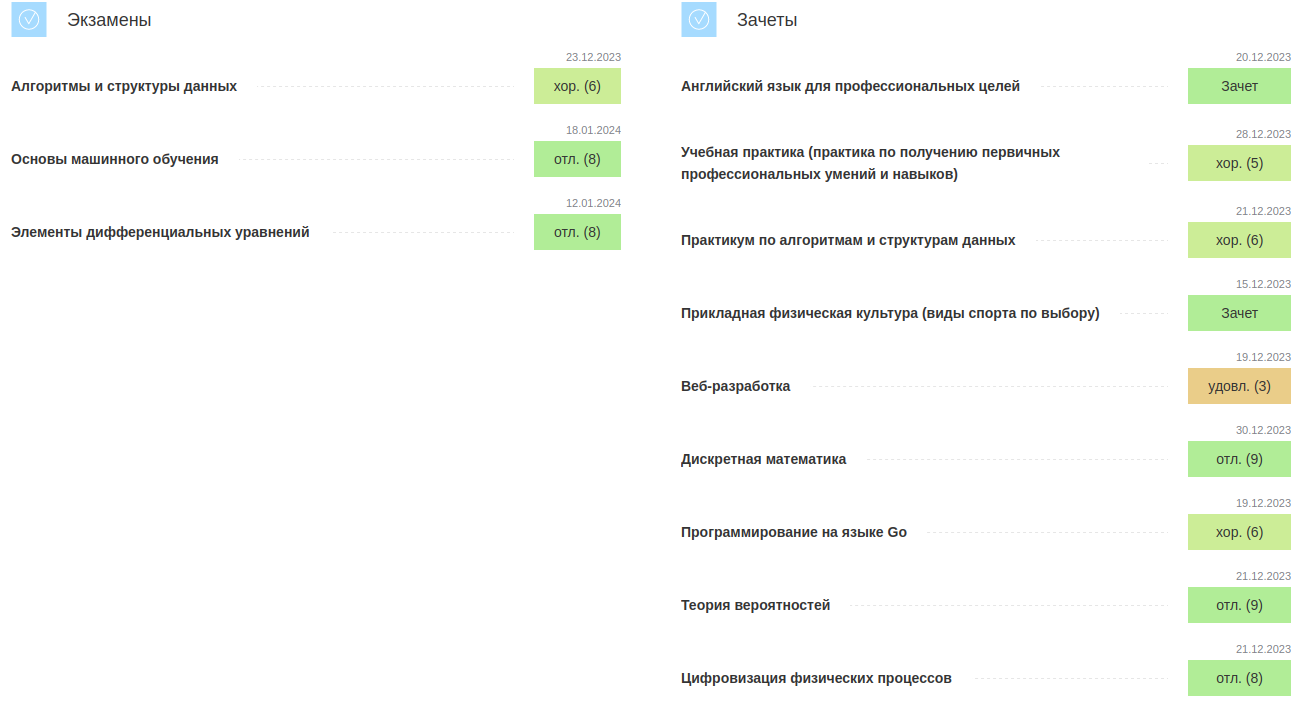
\includegraphics[scale = 0.5]{pic1.png}
  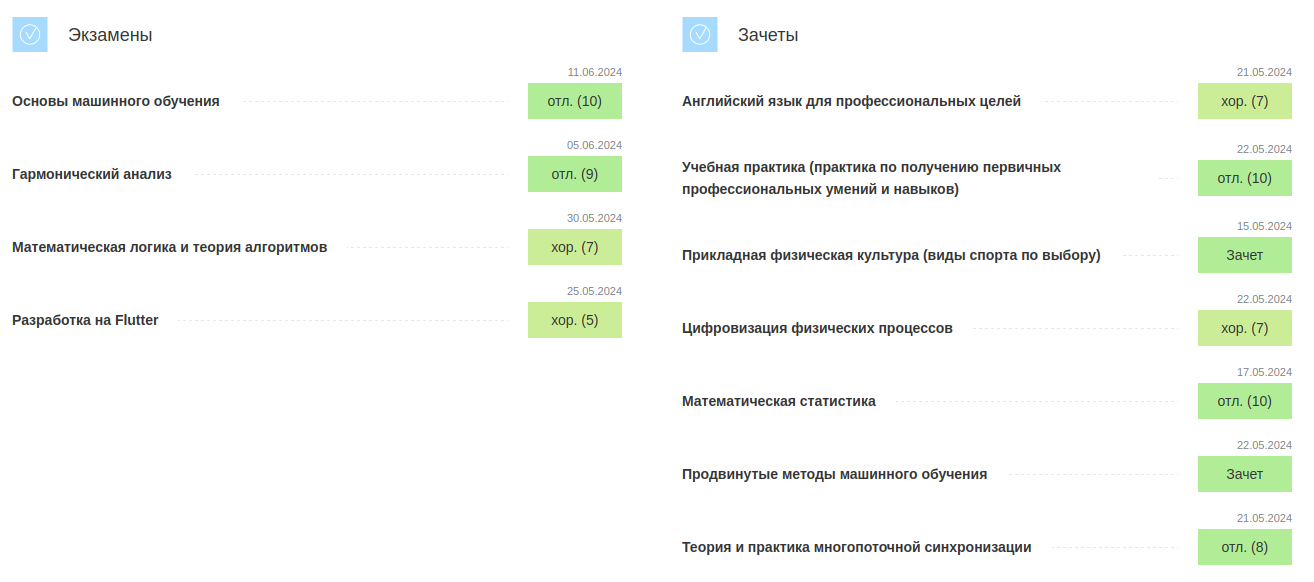
\includegraphics[scale = 0.5]{pic2.png}
\end{center}

\end{document}
